\documentclass[12pt,a4paper]{article}

% ─── Page Layout ───────────────────────────────────────────────────────────────
\usepackage[a4paper, margin=0.8in, headheight=14pt]{geometry}

% ─── Fonts (XeLaTeX) ───────────────────────────────────────────────────────────
\usepackage{fontspec}
\usepackage{unicode-math}
\setmainfont{TeX Gyre Pagella}
\setmonofont[Scale=0.88]{TeX Gyre Cursor}
\setmathfont{Latin Modern Math}

% ─── Packages ──────────────────────────────────────────────────────────────────
\usepackage{xcolor}
\usepackage{colortbl}
\usepackage{titlesec}
\usepackage{enumitem}
\usepackage{tabularx}
\usepackage{booktabs}
\usepackage{array}
\usepackage{amsmath}
\usepackage{tikz}
\usetikzlibrary{shapes.geometric, arrows.meta, positioning, calc, fit}
\usepackage{tcolorbox}
\tcbuselibrary{skins, breakable}
\usepackage{hyperref}
\usepackage{fancyhdr}
\usepackage{graphicx}
\usepackage{microtype}
\usepackage{caption}
\usepackage{setspace}
\usepackage{multirow}
\usepackage{tocloft}

% ─── Q&A helper ────────────────────────────────────────────────────────────────
\newcommand{\Q}[1]{\textbf{#1}\par\noindent\ignorespaces}

% ─── Colour Palette ────────────────────────────────────────────────────────────
\definecolor{myred}{RGB}{196,30,58}
\definecolor{mydark}{RGB}{30,30,50}
\definecolor{mygreen}{RGB}{14,120,80}
\definecolor{myteal}{RGB}{0,130,140}
\definecolor{myamber}{RGB}{180,100,0}
\definecolor{mypurple}{RGB}{100,30,160}
\definecolor{mygray}{RGB}{246,247,249}
\definecolor{mgframe}{RGB}{180,185,200}
\definecolor{watermark}{RGB}{145,150,170}
\definecolor{hdrred}{RGB}{250,232,235}
\definecolor{hdrgreen}{RGB}{220,244,233}
\definecolor{hdrteal}{RGB}{220,242,244}
\definecolor{hdramber}{RGB}{253,242,215}
\definecolor{hdrpurple}{RGB}{238,228,255}
\definecolor{hdrgray}{RGB}{238,240,245}
\definecolor{rowalt}{RGB}{250,251,253}

% ─── Section Formatting ────────────────────────────────────────────────────────
\titleformat{\section}
  {\large\bfseries\color{myred}}{\thesection.}{0.5em}{}
  [\vspace{1pt}{\color{myred}\rule{\linewidth}{0.8pt}}]
\titleformat{\subsection}
  {\normalsize\bfseries\color{myteal}}{\thesubsection}{0.5em}{}
\titlespacing*{\section}{0pt}{18pt}{7pt}
\titlespacing*{\subsection}{0pt}{11pt}{4pt}

\setlength{\parindent}{0pt}
\setlength{\parskip}{4pt}

% ─── TOC Styling ───────────────────────────────────────────────────────────────
\renewcommand{\cfttoctitlefont}{\large\bfseries\color{myred}}
\renewcommand{\cftaftertoctitle}{\par\noindent{\color{myred}\rule{\linewidth}{0.8pt}}}
\setlength{\cftbeforetoctitleskip}{0pt}
\setlength{\cftaftertoctitleskip}{6pt}
\renewcommand{\cftsecfont}{\normalsize\bfseries\color{mydark}}
\renewcommand{\cftsecpagefont}{\normalsize\bfseries\color{mydark}}
\renewcommand{\cftsecleader}{\cftdotfill{\cftdotsep}}
\setlength{\cftbeforesecskip}{7pt}
\renewcommand{\cftsubsecfont}{\small\color{mydark}}
\renewcommand{\cftsubsecpagefont}{\small\color{mydark}}
\setlength{\cftbeforesubsecskip}{3pt}
\setlength{\cftsubsecindent}{1.4em}

% ─── Table helpers ─────────────────────────────────────────────────────────────
\renewcommand{\arraystretch}{1.45}
\setlength{\tabcolsep}{6pt}
\newcolumntype{B}[1]{>{\small\bfseries\raggedright\arraybackslash}p{#1}}

% ─── Header / Footer ───────────────────────────────────────────────────────────
\pagestyle{fancy}
\fancyhf{}
\fancyhead[L]{\small\color{myred}\textbf{EC601}\;\color{mydark}— Control System}
\fancyhead[R]{\small\color{myteal}\textbf{Module 3 Notes}}
\fancyfoot[C]{\small\color{mydark}\thepage}
\fancyfoot[R]{\small\color{watermark}\textit{\copyright\ Biraj}}
\renewcommand{\headrulewidth}{0.5pt}
\renewcommand{\footrulewidth}{0.3pt}

% ─── Hyperref ──────────────────────────────────────────────────────────────────
\hypersetup{
  colorlinks=true, linkcolor=myteal, urlcolor=myteal,
  pdfauthor={Biraj Sarkar},
  pdftitle={EC601 — Module 3 Notes}
}

% ─── tcolorbox styles ──────────────────────────────────────────────────────────
\tcbset{
  tikzbox/.style={
    colback=mygray, colframe=mgframe, boxrule=0.6pt, arc=4pt,
    left=8pt, right=8pt, top=6pt, bottom=6pt,
    colbacktitle=mgframe, coltitle=mydark, fonttitle=\small\bfseries
  },
  defbox/.style={
    colback=hdrgreen, colframe=mygreen, boxrule=0.8pt, arc=4pt,
    left=9pt, right=9pt, top=6pt, bottom=6pt,
    colbacktitle=mygreen, coltitle=white, fonttitle=\small\bfseries
  },
  formulabox/.style={
    colback=hdrteal, colframe=myteal, boxrule=0.8pt, arc=4pt,
    left=9pt, right=9pt, top=7pt, bottom=7pt,
    colbacktitle=myteal, coltitle=white, fonttitle=\small\bfseries
  },
  examplebox/.style={
    colback=hdramber, colframe=myamber, boxrule=0.8pt, arc=4pt,
    left=9pt, right=9pt, top=6pt, bottom=6pt,
    colbacktitle=myamber, coltitle=white, fonttitle=\small\bfseries
  },
  masonbox/.style={
    colback=hdrpurple, colframe=mypurple, boxrule=0.8pt, arc=4pt,
    left=9pt, right=9pt, top=6pt, bottom=6pt,
    colbacktitle=mypurple, coltitle=white, fonttitle=\small\bfseries
  },
  exambox/.style={
    colback=hdrpurple, colframe=mypurple, boxrule=1pt, arc=5pt,
    left=10pt, right=10pt, top=8pt, bottom=8pt,
    colbacktitle=mypurple, coltitle=white, fonttitle=\bfseries,
    breakable
  }
}
% Allow all boxes to break across pages — prevents footer overflow
\tcbset{breakable}

% ─── TikZ styles ───────────────────────────────────────────────────────────────
\tikzset{
  block/.style={rectangle, draw=myteal, fill=hdrteal,
    text width=2.6cm, align=center, minimum height=0.95cm,
    font=\small, rounded corners=3pt, line width=0.7pt},
  wblock/.style={rectangle, draw=myteal, fill=hdrteal,
    text width=3.4cm, align=center, minimum height=0.95cm,
    font=\small, rounded corners=3pt, line width=0.7pt},
  redblock/.style={rectangle, draw=myred, fill=hdrred,
    text width=2.4cm, align=center, minimum height=0.95cm,
    font=\small, rounded corners=3pt, line width=0.7pt},
  polenode/.style={circle, draw=myred, fill=myred,
    minimum size=5pt, inner sep=0pt},
  zeronode/.style={circle, draw=myteal, fill=white,
    minimum size=5pt, inner sep=0pt, line width=1pt},
  sumjunc/.style={circle, draw=myamber, fill=hdramber,
    minimum size=0.62cm, font=\small, line width=0.8pt},
  arrow/.style={-Stealth, thick, color=mydark},
  redarrow/.style={-Stealth, thick, color=myred},
  line/.style={thick, color=mydark},
  axis/.style={-Stealth, thin, color=mydark}
}

% ═══════════════════════════════════════════════════════════════════════════════
\begin{document}
% ═══════════════════════════════════════════════════════════════════════════════

\begin{center}
  {\LARGE\bfseries\color{myred} EC601 — Control System}\\[5pt]
  {\normalsize\color{mydark} Semester VI \quad$\bullet$\quad 3L:0T:0P \quad$\bullet$\quad 3 Credits}\\[3pt]
  {\normalsize\color{myteal}\textbf{Module 3 Exam Notes}}\\[3pt]
  {\small\color{mydark} CGEC \;$|$\; B.Tech ECE (2023--27) \;$|$\; \textit{Biraj Sarkar}}
\end{center}
\vspace{2pt}
\noindent{\color{myred}\rule{\linewidth}{1.5pt}}
\vspace{2pt}

\hypersetup{linkcolor=mydark}
\tableofcontents
\hypersetup{linkcolor=myteal}
\newpage

%═══════════════════════════════════════════════════════════════════════════════
\section{Time Response of Second-Order Systems}
%═══════════════════════════════════════════════════════════════════════════════

A \textbf{second-order system} is the most important standard form in control engineering. Its response to a unit step input exhibits all the key transient characteristics — rise, overshoot, oscillation, and settling — that are used to specify and evaluate system performance.

\begin{tcolorbox}[defbox]
\textbf{Standard Second-Order Transfer Function:}
$$G(s) = \frac{\omega_n^2}{s^2 + 2\zeta\omega_n s + \omega_n^2}$$
where $\omega_n$ = \textbf{natural frequency} (rad/s) and $\zeta$ = \textbf{damping ratio} (dimensionless).\\
The \textbf{characteristic equation} is $s^2 + 2\zeta\omega_n s + \omega_n^2 = 0$.
\end{tcolorbox}

\subsection{Poles of the Second-Order System}

The two closed-loop poles are:
\begin{tcolorbox}[formulabox]
$$s_{1,2} = -\zeta\omega_n \pm \omega_n\sqrt{\zeta^2 - 1}$$
For $0 < \zeta < 1$ (underdamped): $\quad s_{1,2} = -\zeta\omega_n \pm j\,\omega_d$, \quad where $\omega_d = \omega_n\sqrt{1-\zeta^2}$ is the \textbf{damped natural frequency}.
\end{tcolorbox}

\subsection{Damping Cases}

\begin{tabularx}{\linewidth}{|>{\centering\arraybackslash}p{2.2cm}|>{\centering\arraybackslash}p{2.4cm}|X|}
\hline
\rowcolor{hdrteal}
\textbf{\color{myteal}Condition} & \textbf{\color{myteal}Pole Location} & \multicolumn{1}{>{\centering\arraybackslash}X|}{\textbf{\color{myteal}Response}} \\
\hline
$\zeta = 0$ & $\pm j\omega_n$ (imaginary) & Undamped — sustained sinusoidal oscillation \\
\hline
\rowcolor{rowalt}
$0 < \zeta < 1$ & Complex conjugate in LHP & Underdamped — oscillatory, decaying; \textit{most common in practice} \\
\hline
$\zeta = 1$ & Two equal real poles & Critically damped — fastest non-oscillatory response \\
\hline
\rowcolor{rowalt}
$\zeta > 1$ & Two distinct real poles & Overdamped — sluggish, no oscillation \\
\hline
\end{tabularx}

\subsection{Unit Step Response (Underdamped, \texorpdfstring{$\zeta < 1$}{zeta < 1})}

\begin{tcolorbox}[formulabox, title={Step Response Formula}]
$$c(t) = 1 - \frac{e^{-\zeta\omega_n t}}{\sqrt{1-\zeta^2}}\sin\!\left(\omega_d t + \phi\right), \quad t \geq 0$$
where $\phi = \cos^{-1}(\zeta)$ and $\omega_d = \omega_n\sqrt{1-\zeta^2}$.
\end{tcolorbox}

\begin{tcolorbox}[tikzbox, title={Typical Underdamped Step Response}]
\centering
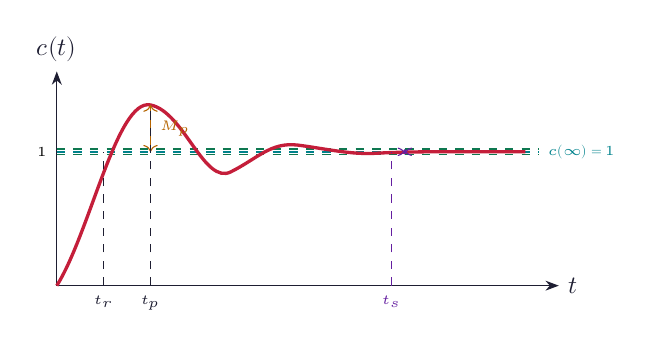
\begin{tikzpicture}[scale=0.85]
  % Axes
  \draw[axis] (0,0) -- (7.5,0) node[right,font=\small] {$t$};
  \draw[axis] (0,0) -- (0,3.2) node[above,font=\small] {$c(t)$};
  % Final value line
  \draw[dashed, color=myteal, line width=0.6pt] (0,2) -- (7.2,2) node[right,font=\tiny,color=myteal] {$c(\infty)=1$};
  % 2% band
  \draw[dashed, color=mygreen, line width=0.5pt] (0,2.04) -- (7.2,2.04);
  \draw[dashed, color=mygreen, line width=0.5pt] (0,1.96) -- (7.2,1.96);
  % Response curve (hand-drawn style)
  \draw[color=myred, line width=1.2pt]
    (0,0) .. controls (0.5,0.8) and (0.9,2.8) .. (1.4,2.7)
    .. controls (1.9,2.6) and (2.2,1.5) .. (2.6,1.7)
    .. controls (3.0,1.9) and (3.2,2.15) .. (3.6,2.1)
    .. controls (4.0,2.05) and (4.4,1.95) .. (4.8,1.98)
    .. controls (5.4,2.01) and (6.0,2.0) .. (7.0,2.0);
  % Annotations
  \draw[<->, color=myamber, thin] (1.4,2) -- (1.4,2.7) node[midway,right,font=\tiny,color=myamber] {$M_p$};
  \draw[dashed, color=mydark, thin] (1.4,0) node[below,font=\tiny] {$t_p$} -- (1.4,2.7);
  \draw[dashed, color=mydark, thin] (0.7,0) node[below,font=\tiny] {$t_r$} -- (0.7,2);
  \draw[<->, color=mypurple, thin] (5.2,1.96) -- (5.2,2.04);
  \draw[dashed, color=mypurple, thin] (5.0,0) node[below,font=\tiny,color=mypurple] {$t_s$} -- (5.0,2);
  \node at (0,2) [left,font=\tiny] {$1$};
\end{tikzpicture}
\end{tcolorbox}

%═══════════════════════════════════════════════════════════════════════════════
\section{Performance Specifications in Time Domain}
%═══════════════════════════════════════════════════════════════════════════════

Time-domain specifications quantify the transient and steady-state behaviour of a system's step response. They are used to set design requirements and evaluate controller performance.

\subsection{Transient Response Specifications}

\begin{tabularx}{\linewidth}{|B{3.0cm}|>{\centering\arraybackslash}p{2.2cm}|X|}
\hline
\rowcolor{hdrteal}
\multicolumn{1}{|>{\centering\arraybackslash}p{3.0cm}|}{\textbf{\color{myteal}Specification}} &
\multicolumn{1}{>{\centering\arraybackslash}p{2.2cm}|}{\textbf{\color{myteal}Symbol}} &
\multicolumn{1}{>{\centering\arraybackslash}X|}{\textbf{\color{myteal}Definition \& Formula}} \\
\hline
Rise Time & $t_r$ & Time for response to rise from 10\% to 90\% of final value (underdamped); or 0\% to 100\% (overdamped). $t_r \approx \dfrac{1.8}{\omega_n}$ \\
\hline
\rowcolor{rowalt}
Peak Time & $t_p$ & Time to reach the first (maximum) peak of overshoot. $t_p = \dfrac{\pi}{\omega_d}$ \\
\hline
Peak Overshoot & $M_p$ & Maximum overshoot above final value, expressed as \%. $M_p = e^{-\pi\zeta/\sqrt{1-\zeta^2}} \times 100\%$ \\
\hline
\rowcolor{rowalt}
Settling Time & $t_s$ & Time for response to stay within $\pm2\%$ (or $\pm5\%$) of final value. $t_s \approx \dfrac{4}{\zeta\omega_n}$ (2\% criterion) \\
\hline
Delay Time & $t_d$ & Time for response to reach 50\% of final value for the first time. $t_d \approx \dfrac{1+0.7\zeta}{\omega_n}$ \\
\hline
\end{tabularx}

\begin{tcolorbox}[formulabox, title={Key Relations — Underdamped 2nd Order}]
\begin{tabularx}{\linewidth}{>{\raggedright\arraybackslash}X >{\raggedright\arraybackslash}X}
$\omega_d = \omega_n\sqrt{1-\zeta^2}$ & Damped natural frequency \\[3pt]
$t_p = \pi/\omega_d$ & Peak time \\[3pt]
$M_p = e^{-\pi\zeta/\sqrt{1-\zeta^2}}\times100\%$ & \% Peak overshoot \\[3pt]
$t_s \approx 4/(\zeta\omega_n)$ & Settling time (2\% band) \\[3pt]
$t_s \approx 3/(\zeta\omega_n)$ & Settling time (5\% band) \\[3pt]
$\zeta = \cos\theta$ & $\theta$ = angle of pole from $-\sigma$ axis
\end{tabularx}
\end{tcolorbox}

\begin{tcolorbox}[exambox, title={Exam Tips — Time Domain Specs}]
\begin{itemize}[leftmargin=*, itemsep=3pt, topsep=0pt]
  \item \textbf{Higher $\omega_n$} → faster response (smaller $t_r$, $t_p$, $t_s$).
  \item \textbf{Higher $\zeta$} → less overshoot, more damping, slower rise.
  \item \textbf{$\zeta = 0.707$} gives $\approx 4.3\%$ overshoot — often used as optimal damping.
  \item \textbf{$M_p$ depends only on $\zeta$}; $t_p$ depends on $\omega_d$; $t_s$ depends on $\zeta\omega_n$.
  \item For a 2nd order system, poles at $s = -\zeta\omega_n \pm j\omega_d$ — draw on $s$-plane for viva.
\end{itemize}
\end{tcolorbox}

%═══════════════════════════════════════════════════════════════════════════════
\section{Steady-State Error and Error Constants}
%═══════════════════════════════════════════════════════════════════════════════

\begin{tcolorbox}[defbox]
\textbf{Steady-State Error:} The difference between the desired reference and the actual output as $t \to \infty$:
$$e_{ss} = \lim_{s \to 0}\, s\,E(s) = \lim_{s \to 0}\, \frac{s\,R(s)}{1 + G(s)H(s)}$$
Valid only when the closed-loop system is \textbf{stable} (Final Value Theorem condition).
\end{tcolorbox}

\subsection{Error Constants}

\begin{tcolorbox}[formulabox, title={Static Error Constants}]
$$K_p = \lim_{s\to 0} G(s)H(s) \quad \text{(Position — for step input)}$$
$$K_v = \lim_{s\to 0}\, s\,G(s)H(s) \quad \text{(Velocity — for ramp input)}$$
$$K_a = \lim_{s\to 0}\, s^2\,G(s)H(s) \quad \text{(Acceleration — for parabolic input)}$$
\end{tcolorbox}

\subsection{SSE vs System Type}

\begin{tabularx}{\linewidth}{|>{\centering\arraybackslash}X|>{\centering\arraybackslash}X|>{\centering\arraybackslash}X|>{\centering\arraybackslash}X|}
\hline
\rowcolor{hdrteal}
\textbf{\color{myteal}Input} & \textbf{\color{myteal}Type 0} & \textbf{\color{myteal}Type 1} & \textbf{\color{myteal}Type 2} \\
\hline
Step $\left(\frac{1}{s}\right)$         & $\dfrac{1}{1+K_p}$ & $0$              & $0$ \\
\hline
\rowcolor{rowalt}
Ramp $\left(\frac{1}{s^2}\right)$       & $\infty$           & $\dfrac{1}{K_v}$ & $0$ \\
\hline
Parabola $\left(\frac{1}{s^3}\right)$   & $\infty$           & $\infty$         & $\dfrac{1}{K_a}$ \\
\hline
\end{tabularx}

\begin{tcolorbox}[exambox, title={Exam Tips — SSE}]
\begin{itemize}[leftmargin=*, itemsep=3pt, topsep=0pt]
  \item \textbf{System type} = number of open-loop poles at $s=0$ (pure integrators).
  \item Increasing gain $K$ reduces SSE but may reduce stability margin.
  \item Adding an integrator (increasing type) eliminates SSE for lower-order inputs.
  \item \textbf{FVT applies only if} $sE(s)$ has all poles in LHP — check stability first.
  \item For non-unity feedback: $e_{ss} = \lim_{s\to0} \dfrac{sR(s)}{1+G(s)H(s)}$.
\end{itemize}
\end{tcolorbox}

%═══════════════════════════════════════════════════════════════════════════════
\section{Root Locus Method}
%═══════════════════════════════════════════════════════════════════════════════

The \textbf{Root Locus} is a graphical method that shows how the closed-loop poles move in the $s$-plane as the open-loop gain $K$ varies from $0$ to $\infty$. It is the most powerful tool for \textbf{controller design} and \textbf{stability analysis}.

\begin{tcolorbox}[defbox]
\textbf{Definition:} The root locus is the locus (path) of the closed-loop poles of the system $T(s) = \dfrac{KG(s)}{1+KG(s)H(s)}$ as $K$ varies from $0$ to $+\infty$.\\[4pt]
\textbf{Characteristic equation:} $1 + KG(s)H(s) = 0 \;\Rightarrow\; G(s)H(s) = -\dfrac{1}{K}$\\[4pt]
\textbf{Angle condition:} $\angle G(s)H(s) = (2q+1)\cdot 180°$, $q = 0,\pm1,\pm2,\ldots$\\[2pt]
\textbf{Magnitude condition:} $|KG(s)H(s)| = 1$
\end{tcolorbox}

\subsection{Rules for Constructing Root Locus}

Let $G(s)H(s) = \dfrac{K\prod(s+z_i)}{\prod(s+p_j)}$ have $m$ zeros and $n$ poles ($n \geq m$).

\begin{tabularx}{\linewidth}{|>{\centering\arraybackslash}p{0.6cm}|B{3.4cm}|X|}
\hline
\rowcolor{hdrteal}
\multicolumn{1}{|>{\centering\arraybackslash}p{0.6cm}|}{\textbf{\color{myteal}\#}} &
\multicolumn{1}{>{\centering\arraybackslash}p{3.4cm}|}{\textbf{\color{myteal}Rule}} &
\multicolumn{1}{>{\centering\arraybackslash}X|}{\textbf{\color{myteal}Statement}} \\
\hline
1 & Number of branches & Equal to $n$ (number of open-loop poles). \\
\hline
\rowcolor{rowalt}
2 & Start \& End points & Locus starts ($K=0$) at open-loop \textbf{poles}; ends ($K\to\infty$) at open-loop \textbf{zeros} (finite or at $\infty$). \\
\hline
3 & Symmetry & Root locus is always \textbf{symmetric about the real axis}. \\
\hline
\rowcolor{rowalt}
4 & Real axis segments & A point on the real axis lies on the locus if the \textbf{total number of real poles and zeros to its right is odd}. \\
\hline
5 & Asymptotes & $(n-m)$ branches go to $\infty$ along asymptotes with angles: $\phi_k = \dfrac{(2k+1)\cdot180°}{n-m}$, $k=0,1,\ldots,(n-m-1)$ \\
\hline
\rowcolor{rowalt}
6 & Centroid of asymptotes & $\sigma_a = \dfrac{\sum\text{poles} - \sum\text{zeros}}{n-m}$ (intersection of asymptotes on real axis) \\
\hline
7 & Breakaway / Break-in & Points where locus leaves/enters real axis. Found from $\dfrac{dK}{ds}=0$, i.e.\ $\dfrac{d}{ds}[G(s)H(s)]=0$. \\
\hline
\rowcolor{rowalt}
8 & $j\omega$-axis crossing & Substitute $s=j\omega$ in characteristic equation; solve for $\omega$ and $K$. (Or use Routh array.) \\
\hline
9 & Angle of departure & From a complex pole $p_k$: $\phi_{dep} = 180° - \sum\angle(p_k - z_i) + \sum\angle(p_k - p_j)$ \\
\hline
\rowcolor{rowalt}
10 & Angle of arrival & At a complex zero $z_k$: $\phi_{arr} = 180° + \sum\angle(z_k - p_j) - \sum\angle(z_k - z_i)$ \\
\hline
\end{tabularx}

\subsection{Root Locus — Worked Example}

\begin{tcolorbox}[examplebox, title={Example: $G(s)H(s) = K/[s(s+2)(s+4)]$}]
\textbf{Given:} $n=3$ poles at $s=0,-2,-4$; $m=0$ zeros.

\textbf{Step 1 — Branches:} 3 branches.

\textbf{Step 2 — Real axis segments:} Right of $s=0$: 0 poles/zeros → not on locus. Between $0$ and $-2$: 1 pole to right → \textbf{on locus}. Between $-2$ and $-4$: 2 poles to right → not on locus. Left of $-4$: 3 poles to right → \textbf{on locus}.

\textbf{Step 3 — Asymptotes:} $n-m=3$, angles $= 60°, 180°, 300°$.

\textbf{Step 4 — Centroid:} $\sigma_a = \dfrac{(0-2-4)-0}{3} = -2$.

\textbf{Step 5 — Breakaway:} $\dfrac{dK}{ds}=0 \Rightarrow 3s^2+12s+8=0 \Rightarrow s \approx -0.845$ (valid, between $0$ and $-2$).

\textbf{Step 6 — $j\omega$ crossing:} Characteristic eq: $s^3+6s^2+8s+K=0$. Routh: $K_{max}=48$, crossing at $\omega=\pm2\sqrt{2}$.
\end{tcolorbox}

\begin{tcolorbox}[tikzbox, title={Root Locus Sketch — $K/[s(s+2)(s+4)]$}]
\centering
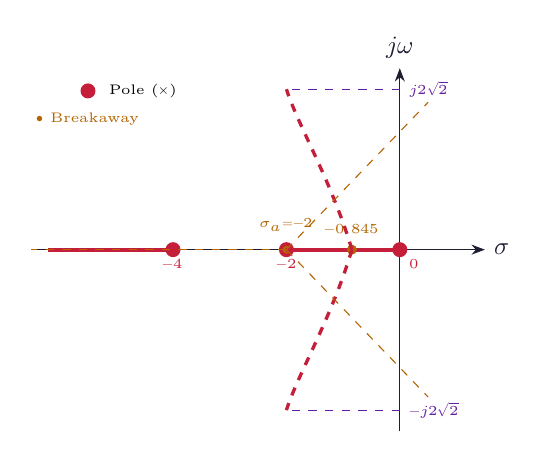
\begin{tikzpicture}[scale=0.72]
  % Axes
  \draw[axis] (-6.5,0) -- (1.5,0) node[right,font=\small] {$\sigma$};
  \draw[axis] (0,-3.2) -- (0,3.2) node[above,font=\small] {$j\omega$};
  % Poles
  \node[polenode] at (0,0) {};   \node[below right,font=\tiny,color=myred] at (0,0) {$0$};
  \node[polenode] at (-2,0) {};  \node[below,font=\tiny,color=myred] at (-2,0) {$-2$};
  \node[polenode] at (-4,0) {};  \node[below,font=\tiny,color=myred] at (-4,0) {$-4$};
  % Centroid
  \node[below,font=\tiny,color=myamber] at (-2,-0.15) {};
  \fill[myamber] (-2,0) circle (2pt);
  \node[above,font=\tiny,color=myamber] at (-2,0.15) {$\sigma_a{=}{-2}$};
  % Real axis locus
  \draw[color=myred, line width=1.4pt] (0,0) -- (-2,0);
  \draw[color=myred, line width=1.4pt] (-4,0) -- (-6.2,0);
  % Breakaway
  \fill[myamber] (-0.845,0) circle (2.5pt);
  \node[above,font=\tiny,color=myamber] at (-0.845,0.1) {$-0.845$};
  % Complex branches (approximate)
  \draw[color=myred, line width=1.2pt, dashed]
    (-0.845,0) .. controls (-1.2,1.2) and (-1.8,2.2) .. (-2,2.83);
  \draw[color=myred, line width=1.2pt, dashed]
    (-0.845,0) .. controls (-1.2,-1.2) and (-1.8,-2.2) .. (-2,-2.83);
  % Asymptote lines (60 deg from centroid)
  \draw[color=myamber, thin, dashed] (-2,0) -- (0.5,2.6);
  \draw[color=myamber, thin, dashed] (-2,0) -- (-6.5,0);
  \draw[color=myamber, thin, dashed] (-2,0) -- (0.5,-2.6);
  % jw crossing
  \draw[dashed, color=mypurple, thin] (0,2.83) node[right,font=\tiny,color=mypurple] {$j2\sqrt{2}$} -- (-2,2.83);
  \draw[dashed, color=mypurple, thin] (0,-2.83) node[right,font=\tiny,color=mypurple] {$-j2\sqrt{2}$} -- (-2,-2.83);
  % Legend
  \node[polenode] at (-5.5,2.8) {}; \node[right,font=\tiny] at (-5.3,2.8) {Pole ($\times$)};
  \node[font=\tiny,color=myamber] at (-5.5,2.3) {$\bullet$ Breakaway};
\end{tikzpicture}
\end{tcolorbox}

\begin{tcolorbox}[exambox, title={Exam Tips — Root Locus}]
\begin{itemize}[leftmargin=*, itemsep=3pt, topsep=0pt]
  \item \textbf{Locus starts at poles, ends at zeros} — memorise this first.
  \item \textbf{Real axis rule:} odd number of poles+zeros to the right → on locus.
  \item \textbf{Centroid formula:} $\sigma_a = (\sum p_i - \sum z_i)/(n-m)$ — very frequently asked.
  \item \textbf{Breakaway point:} solve $dK/ds = 0$ or equivalently $d[G(s)H(s)]/ds = 0$.
  \item \textbf{$j\omega$ crossing:} use Routh array or substitute $s=j\omega$ — gives $K_{max}$ for stability.
  \item \textbf{Gain $K$} at any point on locus: $K = 1/|G(s)H(s)|$ at that $s$.
\end{itemize}
\end{tcolorbox}

%═══════════════════════════════════════════════════════════════════════════════
\section{Compensator Design}
%═══════════════════════════════════════════════════════════════════════════════

A \textbf{compensator} (or controller) is added to the forward or feedback path to reshape the root locus so that the closed-loop poles are placed at desired locations, meeting the time-domain specifications.

\begin{tcolorbox}[defbox]
\textbf{Compensator:} A dynamic element $G_c(s)$ inserted in the control loop to improve transient response, steady-state accuracy, or both. The two fundamental types are \textbf{Lead} (improves transient) and \textbf{Lag} (improves steady-state).
\end{tcolorbox}

%───────────────────────────────────────────────────────────────────────────────
\subsection{Lead Compensator}
%───────────────────────────────────────────────────────────────────────────────

\begin{tcolorbox}[defbox]
\textbf{Lead Compensator:} A compensator whose \textbf{zero is closer to the origin than its pole}. It adds a net \textit{positive} phase angle to the open-loop transfer function, effectively acting like a \textbf{PD controller}. It improves \textbf{transient response} — faster rise time, reduced overshoot.
\end{tcolorbox}

\begin{tcolorbox}[formulabox, title={Lead Compensator Transfer Function}]
$$G_c(s) = K_c\,\frac{s + z_c}{s + p_c}, \qquad p_c > z_c > 0 \quad (\text{pole farther from origin than zero})$$
\textbf{Phase contribution:} $\phi = \angle(s+z_c) - \angle(s+p_c) > 0$ \quad (positive phase lead)\\[4pt]
\textbf{Maximum phase lead:} $\phi_{max} = \sin^{-1}\!\left(\dfrac{1-\alpha}{1+\alpha}\right)$, where $\alpha = z_c/p_c < 1$\\[4pt]
\textbf{Frequency of max lead:} $\omega_{max} = \sqrt{z_c \cdot p_c}$
\end{tcolorbox}

\subsubsection*{Op-Amp Realization of Lead Compensator}

\begin{tcolorbox}[tikzbox, title={Lead Network (RC Circuit)}]
\centering
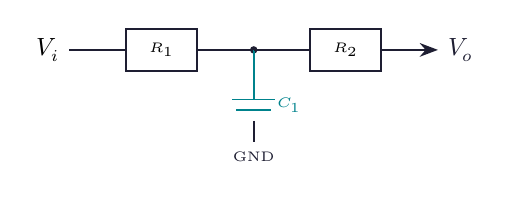
\begin{tikzpicture}[scale=0.9, font=\small]
  % Input
  \draw[line width=0.7pt,color=mydark] (0,1.8) -- (0.8,1.8);
  % R1
  \draw[line width=0.7pt,color=mydark] (0.8,1.5) rectangle (1.8,2.1);
  \node at (1.3,1.8) [font=\tiny] {$R_1$};
  \draw[line width=0.7pt,color=mydark] (1.8,1.8) -- (2.6,1.8);
  % Junction
  \fill[mydark] (2.6,1.8) circle (1.5pt);
  % C1 to ground
  \draw[line width=0.7pt,color=myteal] (2.6,1.8) -- (2.6,1.1);
  \draw[line width=0.7pt,color=myteal] (2.3,1.1) -- (2.9,1.1);
  \draw[line width=0.7pt,color=myteal] (2.35,0.95) -- (2.85,0.95);
  \node at (3.1,1.02) [font=\tiny,color=myteal] {$C_1$};
  \draw[line width=0.7pt,color=mydark] (2.6,0.8) -- (2.6,0.5) node[below,font=\tiny] {GND};
  % R2
  \draw[line width=0.7pt,color=mydark] (2.6,1.8) -- (3.4,1.8);
  \draw[line width=0.7pt,color=mydark] (3.4,1.5) rectangle (4.4,2.1);
  \node at (3.9,1.8) [font=\tiny] {$R_2$};
  \draw[arrow] (4.4,1.8) -- (5.2,1.8) node[right,font=\small] {$V_o$};
  \node at (-0.3,1.8) [font=\small] {$V_i$};
\end{tikzpicture}

\vspace{4pt}
\centering
{\small\color{myteal}$G_c(s)=\dfrac{R_2}{R_1+R_2}\cdot\dfrac{1+sR_1C_1}{1+s\dfrac{R_1R_2}{R_1+R_2}C_1}$}
\end{tcolorbox}

\subsubsection*{Design Procedure (Root Locus)}

\begin{enumerate}[label=\textbf{Step \arabic*:}, leftmargin=2.5cm, itemsep=3pt]
  \item Determine desired closed-loop pole location $s_d$ from specs ($M_p$, $t_s$, $t_p$).
  \item Calculate the \textbf{angle deficiency}: $\phi = 180° - \angle G(s_d)H(s_d)$.
  \item Place the compensator zero $z_c$ and pole $p_c$ such that they contribute angle $\phi$ at $s_d$.
  \item Determine gain $K_c$ from the magnitude condition: $K_c = 1/|G_c(s_d)G(s_d)H(s_d)|$.
  \item Verify SSE and adjust if needed.
\end{enumerate}

%───────────────────────────────────────────────────────────────────────────────
\subsection{Lag Compensator}
%───────────────────────────────────────────────────────────────────────────────

\begin{tcolorbox}[defbox]
\textbf{Lag Compensator:} A compensator whose \textbf{pole is closer to the origin than its zero}. It adds a net \textit{negative} phase angle (phase lag), effectively acting like a \textbf{PI controller}. It improves \textbf{steady-state accuracy} (increases low-frequency gain) without significantly altering the transient response.
\end{tcolorbox}

\begin{tcolorbox}[formulabox, title={Lag Compensator Transfer Function}]
$$G_c(s) = K_c\,\frac{s + z_c}{s + p_c}, \qquad 0 < p_c < z_c \quad (\text{zero farther from origin than pole})$$
\textbf{DC gain boost:} $G_c(0) = K_c\,\dfrac{z_c}{p_c} = K_c\,\beta$, where $\beta = z_c/p_c > 1$\\[4pt]
The lag compensator increases the \textbf{velocity constant} $K_v$ by a factor of $\beta$, reducing SSE.\\[4pt]
\textbf{Placement rule:} Place $z_c$ and $p_c$ very close to the origin (e.g., $z_c = 0.1$, $p_c = 0.01$) so they do not disturb the root locus significantly.
\end{tcolorbox}

\subsubsection*{Op-Amp Realization of Lag Compensator}

\begin{tcolorbox}[tikzbox, title={Lag Network (RC Circuit)}]
\centering
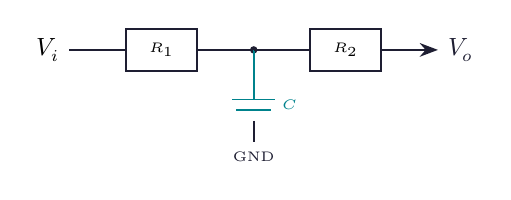
\begin{tikzpicture}[scale=0.9, font=\small]
  % Input wire
  \draw[line width=0.7pt,color=mydark] (0,1.8) -- (0.8,1.8);
  % R1
  \draw[line width=0.7pt,color=mydark] (0.8,1.5) rectangle (1.8,2.1);
  \node at (1.3,1.8) [font=\tiny] {$R_1$};
  \draw[line width=0.7pt,color=mydark] (1.8,1.8) -- (2.6,1.8);
  \fill[mydark] (2.6,1.8) circle (1.5pt);
  % C to ground (below junction)
  \draw[line width=0.7pt,color=myteal] (2.6,1.8) -- (2.6,1.1);
  \draw[line width=0.7pt,color=myteal] (2.3,1.1) -- (2.9,1.1);
  \draw[line width=0.7pt,color=myteal] (2.35,0.95) -- (2.85,0.95);
  \node at (3.1,1.02) [font=\tiny,color=myteal] {$C$};
  \draw[line width=0.7pt,color=mydark] (2.6,0.8) -- (2.6,0.5) node[below,font=\tiny] {GND};
  % R2
  \draw[line width=0.7pt,color=mydark] (2.6,1.8) -- (3.4,1.8);
  \draw[line width=0.7pt,color=mydark] (3.4,1.5) rectangle (4.4,2.1);
  \node at (3.9,1.8) [font=\tiny] {$R_2$};
  \draw[arrow] (4.4,1.8) -- (5.2,1.8) node[right,font=\small] {$V_o$};
  % Input label
  \node at (-0.3,1.8) [font=\small] {$V_i$};
\end{tikzpicture}

\vspace{4pt}
\centering
{\small\color{myteal}$G_c(s)=\dfrac{1+sR_2C}{1+s(R_1+R_2)C}$, \quad pole $<$ zero}
\end{tcolorbox}

\subsubsection*{Design Procedure (Root Locus)}

\begin{enumerate}[label=\textbf{Step \arabic*:}, leftmargin=2.5cm, itemsep=3pt]
  \item Design the uncompensated system to meet transient specs (find required $K$).
  \item Determine the factor $\beta = z_c/p_c$ needed to achieve the desired SSE improvement.
  \item Place $z_c$ and $p_c$ near the origin (e.g., $z_c = 0.1$, $p_c = z_c/\beta$).
  \item Verify that the lag compensator does not significantly shift the dominant poles.
  \item Recalculate gain $K_c$ from magnitude condition at the desired pole.
\end{enumerate}

%───────────────────────────────────────────────────────────────────────────────
\subsection{Lead vs Lag — Comparison}
%───────────────────────────────────────────────────────────────────────────────

\begin{tabularx}{\linewidth}{|B{3.2cm}|>{\centering\arraybackslash}X|>{\centering\arraybackslash}X|}
\hline
\rowcolor{hdrgray}
\multicolumn{1}{|>{\centering\arraybackslash}p{3.2cm}|}{\textbf{Property}} &
\textbf{\color{myred}Lead Compensator} & \textbf{\color{mygreen}Lag Compensator} \\
\hline
Pole-zero relation & $p_c > z_c$ (pole farther) & $p_c < z_c$ (pole closer) \\
\hline
\rowcolor{rowalt}
Phase contribution & Positive (phase lead) & Negative (phase lag) \\
\hline
Equivalent to & PD controller & PI controller \\
\hline
\rowcolor{rowalt}
Primary effect & Improves transient response & Improves steady-state accuracy \\
\hline
Bandwidth & Increases & Decreases slightly \\
\hline
\rowcolor{rowalt}
Noise sensitivity & Higher (differentiating action) & Lower \\
\hline
Root locus effect & Shifts locus to the left (more stable) & Provides gain boost near origin \\
\hline
\rowcolor{rowalt}
Typical use & Fast response needed & Low SSE needed without changing transient \\
\hline
\end{tabularx}

\subsection{Lead-Lag Compensator}

\begin{tcolorbox}[defbox]
\textbf{Lead-Lag Compensator:} Combines both lead and lag sections in cascade to simultaneously improve transient response \textit{and} steady-state accuracy:
$$G_c(s) = K_c\,\frac{(s+z_1)(s+z_2)}{(s+p_1)(s+p_2)}, \quad p_1 > z_1 \text{ (lead)}, \quad p_2 < z_2 \text{ (lag)}$$
Equivalent to a \textbf{PID controller} in terms of effect.
\end{tcolorbox}

\begin{tcolorbox}[exambox, title={Exam Tips — Compensators}]
\begin{itemize}[leftmargin=*, itemsep=3pt, topsep=0pt]
  \item \textbf{Lead:} zero closer to origin than pole → phase lead → faster response.
  \item \textbf{Lag:} pole closer to origin than zero → phase lag → better SSE.
  \item \textbf{Angle deficiency} = $180° - \angle G(s_d)H(s_d)$ — must be provided by lead compensator.
  \item \textbf{$\beta$ factor} for lag = ratio $z_c/p_c$ = SSE improvement factor.
  \item Lead-lag = PID equivalent; used when both transient and SSE specs must be met.
  \item \textbf{RC lead network:} $G_c(s) \propto (1+sR_1C)/(1+s\frac{R_1R_2}{R_1+R_2}C)$ — pole $>$ zero.
  \item \textbf{RC lag network:} $G_c(s) \propto (1+sR_2C)/(1+s(R_1+R_2)C)$ — pole $<$ zero.
\end{itemize}
\end{tcolorbox}

%═══════════════════════════════════════════════════════════════════════════════
% QUICK REVISION — MODULE 3
%═══════════════════════════════════════════════════════════════════════════════
\newpage
\begin{center}
  {\large\bfseries\color{myred} Quick Revision — Module 3}\\[3pt]
  {\small\color{mydark} Time Response, Root Locus \& Compensators $|$ EC601}
\end{center}
\noindent{\color{myred}\rule{\linewidth}{1.2pt}}
\vspace{4pt}

\begin{tcolorbox}[formulabox, title={\textbf{Key Formulas at a Glance}}]
\begin{tabularx}{\linewidth}{B{5.0cm} X}
Standard 2nd order TF      & $G(s) = \omega_n^2/(s^2+2\zeta\omega_n s+\omega_n^2)$ \\[2pt]
Poles                      & $s_{1,2} = -\zeta\omega_n \pm j\omega_d$ \\[2pt]
Damped freq.               & $\omega_d = \omega_n\sqrt{1-\zeta^2}$ \\[2pt]
Peak time                  & $t_p = \pi/\omega_d$ \\[2pt]
\% Peak overshoot          & $M_p = e^{-\pi\zeta/\sqrt{1-\zeta^2}}\times100\%$ \\[2pt]
Settling time (2\%)        & $t_s \approx 4/(\zeta\omega_n)$ \\[2pt]
Settling time (5\%)        & $t_s \approx 3/(\zeta\omega_n)$ \\[2pt]
Rise time (approx.)        & $t_r \approx 1.8/\omega_n$ \\[2pt]
SSE (step, Type 0)         & $1/(1+K_p)$ \\[2pt]
SSE (ramp, Type 1)         & $1/K_v$ \\[2pt]
Asymptote angles           & $\phi_k = (2k+1)\cdot180°/(n-m)$ \\[2pt]
Centroid                   & $\sigma_a = (\sum p_i - \sum z_i)/(n-m)$ \\[2pt]
Gain at point $s_d$        & $K = 1/|G(s_d)H(s_d)|$ \\[2pt]
Lead TF                    & $K_c(s+z_c)/(s+p_c)$, $p_c>z_c$ \\[2pt]
Lag TF                     & $K_c(s+z_c)/(s+p_c)$, $p_c<z_c$ \\[2pt]
Max phase lead             & $\phi_{max}=\sin^{-1}[(1-\alpha)/(1+\alpha)]$, $\alpha=z_c/p_c$
\end{tabularx}
\end{tcolorbox}

\vspace{5pt}

\begin{tcolorbox}[defbox, title={\textbf{One-Line Definitions}}]
\begin{itemize}[leftmargin=*, itemsep=3pt, topsep=0pt]
  \item \textbf{$\omega_n$:} Natural frequency — speed of oscillation without damping.
  \item \textbf{$\zeta$:} Damping ratio — controls oscillation; $\zeta=1$ is critically damped.
  \item \textbf{$\omega_d$:} Damped natural frequency — actual oscillation frequency in underdamped response.
  \item \textbf{Rise time $t_r$:} Time to go from 10\% to 90\% of final value.
  \item \textbf{Peak time $t_p$:} Time to reach first overshoot peak; $t_p = \pi/\omega_d$.
  \item \textbf{Overshoot $M_p$:} Maximum exceedance above final value; depends only on $\zeta$.
  \item \textbf{Settling time $t_s$:} Time to stay within $\pm2\%$ band; $t_s \approx 4/(\zeta\omega_n)$.
  \item \textbf{Root locus:} Path of closed-loop poles as gain $K$ varies $0\to\infty$.
  \item \textbf{Breakaway point:} Point where locus leaves real axis; found from $dK/ds=0$.
  \item \textbf{Centroid:} Intersection of asymptotes on real axis; $\sigma_a = (\sum p - \sum z)/(n-m)$.
  \item \textbf{Lead compensator:} Adds phase lead; improves transient; pole farther than zero.
  \item \textbf{Lag compensator:} Adds phase lag; improves SSE; pole closer than zero.
  \item \textbf{Angle deficiency:} Phase that lead compensator must supply at desired pole location.
\end{itemize}
\end{tcolorbox}

\vspace{5pt}

\begin{tcolorbox}[exambox, title={\textbf{Frequently Asked / Viva Questions}}]
\begin{enumerate}[leftmargin=*, topsep=0pt, label=\textbf{Q\arabic*.}, itemsep=8pt]
  \item \Q{What is the standard second-order transfer function?} $G(s) = \omega_n^2/(s^2+2\zeta\omega_n s+\omega_n^2)$.
  \item \Q{What is the effect of $\zeta$ on step response?} $\zeta<1$: underdamped (oscillatory); $\zeta=1$: critically damped (fastest non-oscillatory); $\zeta>1$: overdamped (sluggish).
  \item \Q{How is $M_p$ related to $\zeta$?} $M_p = e^{-\pi\zeta/\sqrt{1-\zeta^2}}\times100\%$ — depends only on $\zeta$, not $\omega_n$.
  \item \Q{What is the 2\% settling time formula?} $t_s \approx 4/(\zeta\omega_n)$.
  \item \Q{What does the root locus start and end at?} Starts at open-loop poles ($K=0$), ends at open-loop zeros ($K\to\infty$).
  \item \Q{State the real axis rule for root locus.} A point on the real axis is on the locus if the total number of real poles and zeros to its right is odd.
  \item \Q{What is the centroid formula?} $\sigma_a = (\sum\text{poles} - \sum\text{zeros})/(n-m)$.
  \item \Q{How do you find the breakaway point?} Differentiate $K = -1/G(s)H(s)$ with respect to $s$ and set to zero; or solve $d[G(s)H(s)]/ds = 0$.
  \item \Q{What is the difference between lead and lag compensator?} Lead: $p>z$, adds positive phase, improves transient. Lag: $p<z$, adds negative phase, improves SSE.
  \item \Q{What is angle deficiency?} The phase angle that the lead compensator must contribute at the desired closed-loop pole location: $\phi = 180° - \angle G(s_d)H(s_d)$.
  \item \Q{What is the $\beta$ factor in lag compensator?} $\beta = z_c/p_c > 1$; it is the factor by which the velocity constant $K_v$ (and hence SSE improvement) is multiplied.
  \item \Q{What is a lead-lag compensator equivalent to?} A PID controller — provides both transient improvement (lead) and SSE improvement (lag).
\end{enumerate}
\end{tcolorbox}

\vspace{5pt}

\begin{tcolorbox}[tikzbox, title={\textbf{Damping Cases — Quick Reference}}]
\begin{tabularx}{\linewidth}{|>{\centering\arraybackslash}X|>{\centering\arraybackslash}X|>{\centering\arraybackslash}X|}
\hline
\rowcolor{hdrteal}
\textbf{\color{myteal}$\zeta$ value} & \textbf{\color{myteal}Pole type} & \textbf{\color{myteal}Response} \\
\hline
$\zeta = 0$ & $\pm j\omega_n$ & Undamped — sustained oscillation \\
\hline
\rowcolor{rowalt}
$0 < \zeta < 1$ & Complex conjugate & Underdamped — decaying oscillation \\
\hline
$\zeta = 1$ & Two equal real & Critically damped — fastest non-oscillatory \\
\hline
\rowcolor{rowalt}
$\zeta > 1$ & Two distinct real & Overdamped — no oscillation, slow \\
\hline
\end{tabularx}
\end{tcolorbox}

\vspace{5pt}

\begin{tcolorbox}[tikzbox, title={\textbf{Root Locus Rules — Quick Reference}}]
\begin{tabularx}{\linewidth}{|>{\centering\arraybackslash}p{0.5cm}|B{3.2cm}|X|}
\hline
\rowcolor{hdrteal}
\textbf{\color{myteal}\#} & \multicolumn{1}{>{\centering\arraybackslash}p{3.2cm}|}{\textbf{\color{myteal}Rule}} & \multicolumn{1}{>{\centering\arraybackslash}X|}{\textbf{\color{myteal}Formula / Statement}} \\
\hline
1 & Branches & $n$ branches (= no.\ of poles) \\
\hline
\rowcolor{rowalt}
2 & Start/End & $K=0$: poles; $K\to\infty$: zeros \\
\hline
3 & Symmetry & Symmetric about real axis \\
\hline
\rowcolor{rowalt}
4 & Real axis & Odd poles+zeros to the right \\
\hline
5 & Asymptote angles & $(2k+1)\cdot180°/(n-m)$ \\
\hline
\rowcolor{rowalt}
6 & Centroid & $(\sum p_i - \sum z_i)/(n-m)$ \\
\hline
7 & Breakaway & $dK/ds = 0$ \\
\hline
\rowcolor{rowalt}
8 & $j\omega$ crossing & $s=j\omega$ in char.\ eq.\ or Routh \\
\hline
\end{tabularx}
\end{tcolorbox}

\end{document}
